% Reviewer 2

\reviewer

\begin{generalcomment}
    \textbf{General Comments:} The paper offers an extensive overview of the latest confidence calibration techniques for deep imbalanced learning, presenting significant and relevant research. However, there are a few areas where improvement could be made.
   
    \textbf{Strengths:} (i) xxx; (ii) xxx; (iii) xxx.

    \textbf{Areas for Improvement:} (i) xxx; (ii) xxx. 
     
    \textbf{Weaknesses:} (i) xxx; (ii) xxx. 

\end{generalcomment}
\begin{revmeta}[]
	We would like to express our sincere gratitude for your feedback and valuable suggestions on our manuscript. We have carefully considered each of your points and revised them carefully.
\end{revmeta}

\begin{revcomment}
A summary of the practical domains where these methods have been applied, or could be applied, is missing.
\end{revcomment}
\begin{revresponse}[]
	Thank you for the pertinent suggestions. We agree with your point of view. We added an application section (Section VIII) on the 18th page of the revised manuscript. For your convenience, we put the newly added application section below, and we hope it will satisfy you.
	
	\begin{table}[H]
    \centering
    \caption{Example of a three-line table.}
    \begin{tabular}{lccc}
    \toprule
    Item & Metric A & Metric B & Metric C \\
    \midrule
    Sample 1 & 12.3 & 45.6 & 78.9 \\
    Sample 2 & 9.8  & 23.4 & 56.7 \\
    \bottomrule
    \end{tabular}
    \label{tab:table2}
\end{table}
    
	\lipsum[4] \cite{gao2022comparative,zidonghua} The table is shown in Table~\ref{tab:table2}.

    \begin{algorithm}[H]
    \begin{addedenv}
    \caption{Reservoir Sampling (Generated by AI)}
    \label{algo:reservoir}
    \begin{algorithmic}[1]
      \Require Stream of items $x_1, x_2, \ldots$ (length unknown), reservoir size $m$
      \Ensure A uniform random sample $R$ of size $m$ from the stream
      \State Initialize empty reservoir $R$
      \For{$t \gets 1$ \textbf{to} $m$}
        \State $R_t \gets x_t$ \Comment{Fill the reservoir with the first $m$ items}
      \EndFor
      \State $t \gets m$
      \While{next item $x$ arrives}
        \State $t \gets t + 1$
        \State Draw $j \sim \mathrm{Uniform}\{1,2,\ldots,t\}$
        \If{$j \le m$}
          \State $R_j \gets x$ \Comment{Replace item $j$ with probability $m/t$}
        \EndIf
      \EndWhile
      \State \Return $R$
    \end{algorithmic}
    \end{addedenv}
  \end{algorithm}
  
    \lipsum[5][1-2] \added{The algorithm is shown in Algorithm~\ref{algo:reservoir}.}

    We have added the following changes into our revised manuscript:
	\begin{changes}
	
		\lipsum[2][1-2] \cite{silva2023classifier,AnExperimentalInvestigation} \added{We have added the new results. \lipsum[2][3-5]. See Figure~\ref{fig:sample_figure1}.}

		\begin{figure}[H]
    \centering
    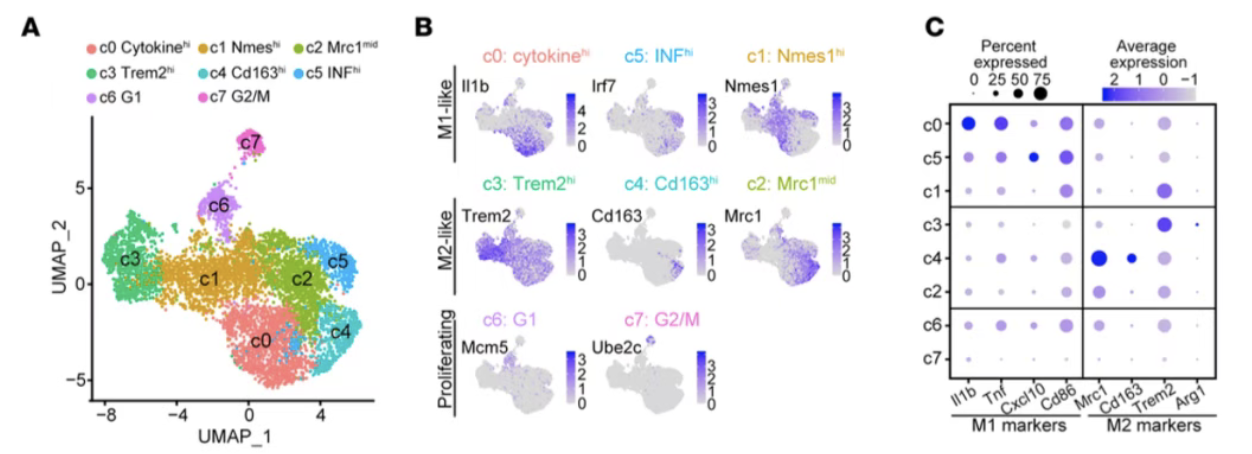
\includegraphics[width=\textwidth,keepaspectratio]{utils/imgs/sample1.png}
    \caption{sample figure}
    \label{fig:sample_figure1}
\end{figure}
		\newpage
		\modified{\lipsum[3]} \added{The results are shown in Table~\ref{tab:table1}. }
		% Requires: \usepackage{booktabs}
\begin{table}[H]
    \centering
    \begin{addedenv}
    \caption{Example table (header + two data rows).}
    \label{tab:table1}
    \begin{tabular}{lcccc}
    \toprule
    Item & Feature 1 & Feature 2 & Feature 3 & Feature 4 \\
    \midrule
    Sample 1 & 12.4 & 0.86 & 45 & 7.9 \\
    Sample 2 & 10.1 & 0.73 & 39 & 8.4 \\
    \cellcolor[HTML]{F9D7EF}Ours & \cellcolor[HTML]{F9D7EF}11.2 & \cellcolor[HTML]{F9D7EF}0.78 & \cellcolor[HTML]{F9D7EF}42 & \cellcolor[HTML]{F9D7EF}8.1 \\
    \bottomrule
    \end{tabular}
    \end{addedenv}
\end{table}
    
		
	\end{changes}
	
\end{revresponse}

\begin{revcomment}
The paper is not clear about the application of the proposed methods.
\end{revcomment}
\begin{revresponse}[]
    Thank you for your constructive suggestions. \lipsum[6] \cite{tomsett2020rapid,liu2019large,qi2023text} The figure is shown in Figure~\ref{fig:sample_figure2}.
    \begin{figure}[H]
    \centering
    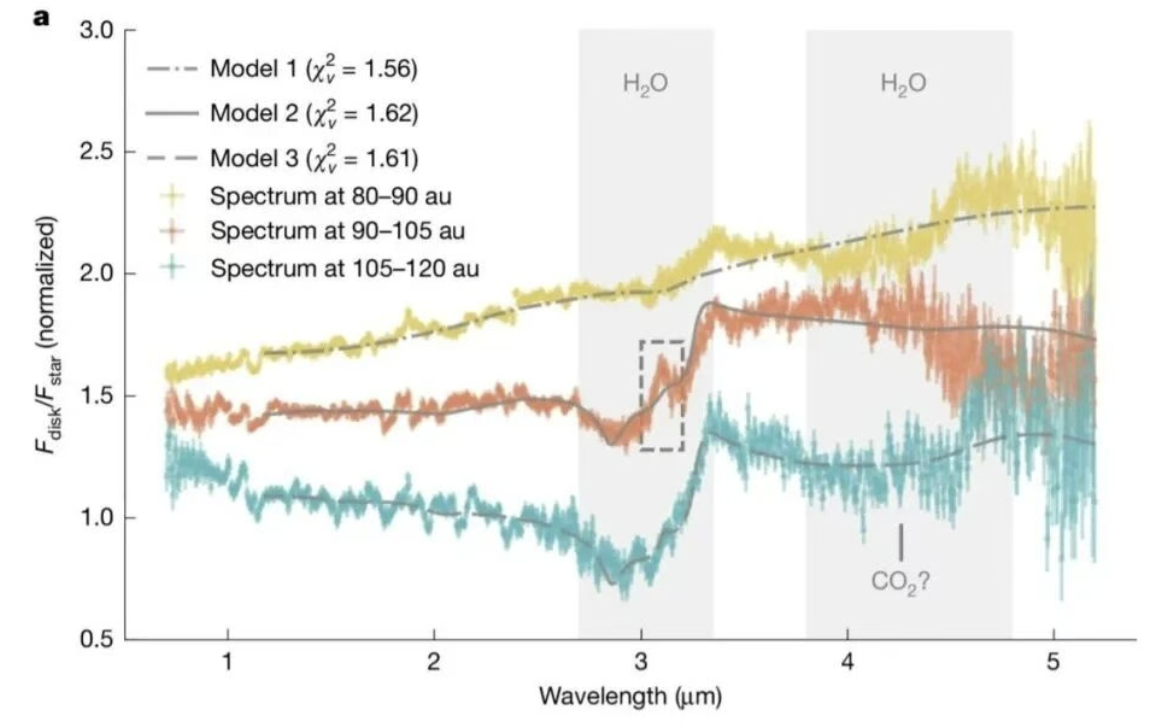
\includegraphics[width=0.8\textwidth,keepaspectratio]{utils/imgs/sample2.png}
    \caption{sample figure 2}
    \label{fig:sample_figure2}
\end{figure}

    \lipsum[7] \cite{zhang2023deep,fu2022long} The algorithm is shown in Algorithm~\ref{algo:dsu}.
    \begin{algorithm}[H]
    \caption{Disjoint Set Union (Union--Find) with Path Compression and Union by Rank (Generated by AI)}
    \label{algo:dsu}
    \begin{algorithmic}[1]
      \Require A finite set $U = \{1,\dots,n\}$; a list of union operations
      \Ensure Ability to query whether two elements are in the same set
      \Statex
      \Function{MakeSet}{$n$}
        \For{$i \gets 1$ \textbf{to} $n$}
          \State parent[$i$] $\gets i$
          \State rank[$i$] $\gets 0$
        \EndFor
      \EndFunction
      \Statex
      \Function{Find}{$x$}
        \If{parent[$x$] $\ne x$}
          \State parent[$x$] $\gets$ \Call{Find}{parent[$x$]} \Comment{Path compression}
        \EndIf
        \State \Return parent[$x$]
      \EndFunction
      \Statex
      \Function{Union}{$x, y$}
        \State $rx \gets$ \Call{Find}{$x$}; \quad $ry \gets$ \Call{Find}{$y$}
        \If{$rx = ry$} \State \Return \EndIf
        \If{rank[$rx$] $<$ rank[$ry$]}
          \State parent[$rx$] $\gets ry$
        \ElsIf{rank[$rx$] $>$ rank[$ry$]}
          \State parent[$ry$] $\gets rx$
        \Else
          \State parent[$ry$] $\gets rx$; \quad rank[$rx$] $\gets$ rank[$rx$] $+ 1$
        \EndIf
      \EndFunction
      \Statex
      \Function{SameSet}{$a, b$}
        \State \Return \Call{Find}{$a$} $=$ \Call{Find}{$b$}
      \EndFunction
    \end{algorithmic}
  \end{algorithm}
  

\end{revresponse}

\clearpage
\printbibliography[heading=bibintoc, heading=bibliography, title={References}, section=\therefsection]